\documentclass[conference]{IEEEtran}

\usepackage{amsmath}
\usepackage{fontspec}
\usepackage{newtxtext,newtxmath}
\newfontfamily\tamilfont[Path=/usr/share/fonts/noto/,Script=Tamil,Extension=.ttf,UprightFont=NotoSansTamil-Regular,BoldFont=NotoSansTamil-Bold]{NotoSansTamil-Regular}
\newcommand{\tamil}[1]{{\tamilfont #1}}
\usepackage{graphicx}
\graphicspath{{../figures/}}
\usepackage{booktabs}
\usepackage{cleveref}
\usepackage{microtype}
\usepackage[backend=biber,style=ieee,maxbibnames=3,minbibnames=1]{biblatex}
\addbibresource{../refs.bib}

\begin{document}

\title{Robustness of Character-Level Transliteration to\\
Informal Typing in Romanized Tamil}

\makeatletter
\newcommand{\linebreakand}{\end{@IEEEauthorhalign}\hfill\mbox{}\par\mbox{}\hfill\begin{@IEEEauthorhalign}}
\makeatother
\author{
\IEEEauthorblockN{Lebi Raja}
\IEEEauthorblockA{\textit{Division of Data Science and Cybersecurity}\\
\textit{Karunya Institute of Technology and Sciences}\\
India}
\and
\IEEEauthorblockN{KRM Lohith}
\IEEEauthorblockA{\textit{Division of Data Science and Cybersecurity}\\
\textit{Karunya Institute of Technology and Sciences}\\
India}
\linebreakand
\IEEEauthorblockN{Allen John Isac}
\IEEEauthorblockA{\textit{Division of Data Science and Cybersecurity}\\
\textit{Karunya Institute of Technology and Sciences}\\
India}
\and
\IEEEauthorblockN{KP Shohil}
\IEEEauthorblockA{\textit{Division of Data Science and Cybersecurity}\\
\textit{Karunya Institute of Technology and Sciences}\\
India}
}

\maketitle

\begin{abstract}
People type Tamil in Latin letters, yet transliteration models are trained and tested on carefully romanized text, so their accuracy under fast, informal typing is unknown.
We release a paired, seeded benchmark of seven Tamil-specific noise operators at four severities, built from the Dakshina test lexicon, and evaluate 110 character-level models (BiLSTM with attention and Transformer, 1M to 8M parameters, five seeds).
Our implementation reproduces the published development CER of 8.4.
Vowel dropping and keyboard slips raise character error rate (CER) from about 9 to 22--24 at severity 0.3; the other operators cost 1 to 3 points.
Tamil-phonological noise training cuts BiLSTM vowel-drop CER from 24.0 to 17.7 but does not transfer to a held-out operator; adding sampled back-transliterations gives the lowest mixed-noise CER (21.8 against 25.5).
Fine-tuning that Transformer on 2.4M pairs gives a 12.6\,MB model with mixed-noise CER 17.8 at unchanged clean accuracy.
\end{abstract}

\begin{IEEEkeywords}
transliteration, Tamil, robustness, data augmentation, sequence-to-sequence, romanization
\end{IEEEkeywords}

%% ------------------------------------------------------------------
\section{Introduction}
Type \emph{vanakkam, eppadi irukkinga?} into a phone and you have written a Tamil greeting (\tamil{வணக்கம், எப்படி இருக்கிறீர்கள்?}) without a single Tamil letter.
Many Tamil speakers write this way in messages and search boxes, because a Latin keyboard is always at hand.
Keyboards, search engines and chat assistants then have to turn the Latin spelling back into Tamil script, a task called transliteration: sounds are mapped to letters, not meanings to words.
It is hard because the Latin alphabet cannot express several Tamil distinctions (vowel length, doubled consonants, and the several n, l and r sounds), so one word has many spellings; annotators of the Dakshina corpus produced 2.7 romanizations per word on average~\cite{roark2020dakshina}.
Fast typing adds more: dropped vowels (\emph{kankl} for \emph{kanakkil}), shortened long vowels, collapsed double letters, stretched letters (\emph{semmaaa}) and key slips~\cite{wolfsonkin2019latin,herath2024tamzhi}.

Small character-level neural models already reach about 8--9\% character error rate (CER) on the Dakshina Tamil lexicon~\cite{roark2020dakshina,kirov2024context}.
That text, however, is formal and was romanized word by word with care, and the same holds for the larger mined corpus Aksharantar~\cite{madhani2023aksharantar}.
Where informal input has been tested, accuracy falls sharply: a Malayalam model goes from 7.4 to 22.7 CER on vowel-omitted words~\cite{baiju2024malayalam}, and on 100 hand-noised Tamil words most systems fall to about 20\% top-1~\cite{azam2025beyond}.
The only Tamil evaluation on naturally typed input that we found uses a proprietary test set~\cite{hellsten2017keyboard}.

We address two gaps.
\textbf{G1:} there is no public benchmark that pairs clean and noisy versions of the same Tamil test words, with a per-phenomenon breakdown and graded severity.
\textbf{G2:} it is unclear which training remedy helps, and whether a remedy trained on some error types protects against others.
Our contributions are:
(1)~a seeded, paired benchmark of seven Tamil noise operators at four severities over the 6{,}833 distinct Dakshina test inputs;
(2)~a controlled comparison of six training conditions, including a control that separates ``more words'' from ``more spelling variety'' and two held-out-operator variants;
(3)~a size-matched, equally tuned comparison of a BiLSTM and a Transformer at three sizes with five seeds, as a supporting result;
and (4)~a code and log release and a single 12.6\,MB deployment model.
Dropped vowels and keyboard slips do most of the damage; Tamil-aware noise training removes much of the vowel-drop damage but only for the operators it models; and extra data matters at least as much as spelling variety (\Cref{sec:results}).

%% ------------------------------------------------------------------
\section{Related Work}
We group earlier work by model family and note what each leaves open for our two gaps (\Cref{tab:related}).

\textbf{Rule-based and statistical systems.}
Brahmi-Net combines rules and statistical translation for many Indian languages~\cite{kunchukuttan2015brahminet}.
The only Tamil evaluation on naturally typed phone input that we found is a finite-state keyboard model (WER 26.2 to 22.6), but its test set is not public~\cite{hellsten2017keyboard}.
Wolf-Sonkin et al.\ catalogue romanization variation such as optional aspiration and vowel doubling~\cite{wolfsonkin2019latin}, and TAMZHI derives Tamil shorthand rules from a 215-user survey, scoring 93\% character and 70\% word accuracy on 700 items without a neural comparison~\cite{herath2024tamzhi}.

\textbf{Neural models.}
Dakshina supplies Tamil romanization lexicons and strong BiLSTM and Transformer baselines~\cite{roark2020dakshina}; a 25-seed study finds the Transformer slightly ahead (8.2 against 8.6 CER), reversing the earlier ranking~\cite{kirov2024context}.
Aksharantar scales to 26 million mined pairs and lifts Tamil top-1 from 56.0 to 67.7~\cite{madhani2023aksharantar}, but its annotators were told to avoid frivolous variants, so it too is cleaner than chat text.
Multilingual Indic models suffer from Tamil's under-specified script~\cite{kunchukuttan2021largescale,kunchukuttan2018orthographic}.
Informal-typing results exist for Malayalam, where a BiLSTM triples its CER on vowel-omitted input~\cite{baiju2024malayalam,sumanathilaka2025indonlp}, but not for Tamil and without graded severity.
LSTM-versus-Transformer comparisons on character tasks are confounded by parameter count and batch size~\cite{moran2020effective,wu2021applying}.

\textbf{Pretrained and large language models.}
Large language models reach 76.6\% top-1 on clean Dakshina Tamil, yet most systems, including IndicXlit, fall to about 20\% on 100 hand-noised words (a fine-tuned GPT-4o reaches 37\%)~\cite{azam2025beyond}.
Byte-level pretrained models are robust to some character noise~\cite{xue2022byt5} but were unstable on Tamil without data pruning~\cite{kirov2024context}.

\textbf{Noise and augmentation.}
Models trained on one noise type transfer poorly to others~\cite{belinkov2018synthetic}; a balanced mixture of typo-like noise helps at little clean cost but not for stylistic variation~\cite{karpukhin2019training}; and for romanized language identification, sampled spelling variants beat larger models, while machine-romanized test data overstate accuracy~\cite{benton2025romanizedlid,madhani2023bhasha}.
Back-translation is the standard route to synthetic parallel data~\cite{sennrich2016backtranslation}.
None of these was tested for Tamil word transliteration, which is the focus of our work.

\begin{table*}[t]
\caption{Closest earlier work and what it leaves open (strengths as reported by the cited papers).}
\label{tab:related}
\centering\footnotesize
\begin{tabular}{llp{4.3cm}p{6.3cm}}
\toprule
Family & Work & Strength & Left open for Tamil \\
\midrule
Rule/statistical & Brahmi-Net~\cite{kunchukuttan2015brahminet} & Rules plus statistical MT, many pairs & No test of informal typing \\
 & Hellsten et al.~\cite{hellsten2017keyboard} & On-device, real typed Tamil test & Test set proprietary, not reproducible \\
 & TAMZHI~\cite{herath2024tamzhi} & Shorthand rules from 215 users & 700 items, no neural comparison \\
Neural & Roark et al.~\cite{roark2020dakshina} & Dakshina data, BiLSTM/Transformer baselines & Clean, formal text; five seeds \\
 & Kirov et al.~\cite{kirov2024context} & 25 seeds, context, ensembles & Clean input only; ranking reverses Roark \\
 & Madhani et al.~\cite{madhani2023aksharantar} & 26M pairs, large clean gain & About one romanization per word; clean \\
 & Baiju et al.~\cite{baiju2024malayalam} & Shows ad-hoc drop (7.4 to 22.7 CER) & Malayalam; one noise type, no severity \\
LLM/pretrained & Azam et al.~\cite{azam2025beyond} & LLM and IndicXlit benchmark & Only 100 hand-noised Tamil words, unpaired \\
 & Xue et al.~\cite{xue2022byt5} & Byte-level robustness & Not studied for informal Tamil romanization \\
Noise & Belinkov \& Bisk~\cite{belinkov2018synthetic} & Noise types do not transfer & Not transliteration, not Tamil \\
\bottomrule
\end{tabular}
\end{table*}

%% ------------------------------------------------------------------
\section{Proposed Methodology}
\label{sec:method}

\subsection{Data and paired noise benchmark}
\textbf{Clean data.}
We use the Dakshina Tamil romanization lexicon: 25{,}000 training words (68{,}218 romanization pairs), 2{,}500 development words (6{,}827 pairs) and 2{,}500 test words (6{,}864 pairs), word-disjoint~\cite{roark2020dakshina}.
Inputs are lowercase Latin and outputs NFC-normalised Tamil; a romanization attested for several native forms is scored against all of them.
The development set is used only for early stopping and tuning, and the test lexicon holds 6{,}833 distinct romanized inputs.

\textbf{Independent test sets.}
Aksharantar's Tamil test file contains every Dakshina test pair~\cite{madhani2023aksharantar}, so we keep only rows whose native word occurs in no Dakshina split.
This leaves three subsets by source, AK-Freq (2{,}607 distinct inputs), AK-NEI (991) and AK-NEF (706), and their union AK-all.
Aksharantar's training file shares stems with Dakshina test words, so the controlled experiments never train on it.

\textbf{Noise operators.}
Seven operators perturb the romanized input only (\Cref{tab:ops}), each at severity $p\in\{0.1,0.2,0.3,0.5\}$, giving 28 noisy copies of the test inputs.
The random seed is derived from the word, operator and severity, so the sets are exactly reproducible and each noisy item stays paired with its clean form and references.
V-DROP deletes non-initial vowels; V-LEN and GEM collapse long vowels and doubled consonants; DIGRAPH swaps th/t, dh/d, sh/s, ch/c,s and maps zh to l or z; KEY replaces a letter with a neighbour on the keyboard; REPEAT stretches a letter; MIX combines the six.
Operators are motivated by the typing phenomena in the literature~\cite{wolfsonkin2019latin,herath2024tamzhi,belinkov2018synthetic}.
In our own count on public code-mixed Tamil comments~\cite{chakravarthi2020tamilmix} (heuristic, not checked by hand) vowel dropping, vowel-length collapse and stretching occur several times more often than in Dakshina, while dropped h does not, so DIGRAPH is only partly symmetric.
Because $p$ is a per-position probability, \Cref{tab:ops} reports the share of words changed; at $p{=}0.3$ the character edit rate is 12.7\% for V-DROP, 7.4\% for KEY and 15.8\% for MIX.

\begin{table}[t]
\caption{Noise operators and the share of test words they change (\%) at three severities.}
\label{tab:ops}
\centering\footnotesize
\resizebox{\columnwidth}{!}{\begin{tabular}{llccc}
\toprule
Operator & Effect & \multicolumn{3}{c}{Words changed (\%) at $p=$} \\
\cmidrule(lr){3-5}
 & & 0.1 & 0.3 & 0.5 \\
\midrule
V-DROP & delete non-initial vowels & 34 & 73 & 89 \\
V-LEN & collapse doubled vowels & 4 & 13 & 21 \\
GEM & collapse doubled consonants & 3 & 9 & 15 \\
DIGRAPH & th/t, dh/d, sh/s, ch/c/s swaps; zh$\to$l,z & 12 & 32 & 47 \\
KEY & adjacent QWERTY key substitution & 21 & 52 & 69 \\
REPEAT & stretch one vowel by 1--3 letters & 10 & 29 & 51 \\
MIX & random combination of the six & 35 & 69 & 82 \\
\bottomrule
\end{tabular}}
\end{table}

\subsection{Training conditions}
To study G2 we train both architectures under eight conditions.
A0 uses Dakshina only.
A1 adds random character noise (deletion, insertion, substitution, swap)~\cite{karpukhin2019training}.
A2 adds the four Tamil-phonological operators V-DROP, V-LEN, GEM and DIGRAPH.
A3 adds sampled back-transliterations~\cite{sennrich2016backtranslation}, and A4 combines A2 and A3.
CTRL adds the same words as A3 romanized once, greedily, so A3 against CTRL separates spelling variety from extra words.
A2-noGEM and A2-noVDROP omit one operator from A2 and are tested on it.
KEY and REPEAT are deliberately absent from A2, so they test transfer.
Online noise is re-drawn every epoch and leaves 40\% of items clean.

The back-transliteration pool has 60{,}000 further Tamil words taken from the IndicXlit unigram list.
We removed every Dakshina word, every independent-test word and any word sharing a five-code-point prefix with a held-out word (46{,}652 of 137{,}748 candidates were removed for stem overlap alone).
A Tamil-to-Latin BiLSTM trained on Dakshina romanizes each word three times by sampling at temperature 1; a closeness filter against its greedy output drops 17{,}828 degenerate samples and leaves 123{,}488 pairs.
These romanizations are machine-made and carry the errors of that model.

\subsection{Models, training and metrics}
Both models are character-level with separate source and target vocabularies (30 and 52 symbols).
The BiLSTM has a two-layer bidirectional encoder, a two-layer decoder and Luong attention~\cite{luong2015effective,bahdanau2015neural}; the Transformer is a pre-LN encoder-decoder with three layers per side and four heads~\cite{vaswani2017attention}.
Widths give about 1M, 3M and 8M parameters (BiLSTM 0.98M, 2.99M, 8.04M; Transformer 0.80M, 3.15M, 8.70M), so ``matched'' means approximately matched.
Training uses Adam with gradient clipping at 1.0 and early stopping on development CER.
For each architecture and size, 20 random-search trials vary learning rate, batch size (64--512), dropout, label smoothing and, for the Transformer, warmup; selection uses development CER only, and the test set is never used for selection.
Decoding is beam search with beam 10.

CER is the corpus-level Levenshtein distance over code points between the top hypothesis and the closest attested reference, divided by reference length~\cite{roark2020dakshina,kirov2024context}.
Top-$k$ accuracy counts an input correct if any of the best $k$ hypotheses equals any reference, and MRR uses the rank of the first correct one~\cite{chen2018news}.
Each cell is the mean and sample standard deviation over five seeds.
Systems are compared with a paired bootstrap over test items (10{,}000 resamples), and the six main conditions with Kruskal--Wallis and Dunn's test with Holm correction on per-seed CER.
With five seeds the seed-level tests have little power, and the item bootstrap describes the test set, not the population of trainings.

\subsection{Implementation and reproducibility}
All models use PyTorch 2.11 (CUDA 12.8) on one RTX 5070 (12\,GB) shared by up to three jobs; the whole study (120 tuning trials, 30 comparison runs, 80 augmentation runs) took about a day of wall time.
Every run writes a JSON file with its configuration, seed, code commit, data checksums and all metrics, and every number in this paper is generated from those files by scripts in the repository.
The 110 final checkpoints were re-scored per item; a model that does not reproduce its logged score is flagged.

\subsection{Deployment model}
For use we also build one model.
We fine-tune \emph{all} 3.15M weights of the best-seed A4 Transformer, with no adapters and no frozen layers, on 2.41M pairs per epoch: Dakshina train three times, the 123{,}488 back-transliterated pairs, and 2.08M Aksharantar pairs.
From the mined Aksharantar rows we dropped those whose round-trip quality score is below $-0.10$ (the authors' own threshold is $-0.35$) and every word of the Dakshina and independent test sets.
Noise from all six operators is applied online to half of the items.
We use Adam at learning rate $10^{-4}$ with cosine decay, batch size 512, label smoothing 0.1 and five epochs (20 minutes), and keep the epoch with the best mean of clean and mixed-noise development CER.

%% ------------------------------------------------------------------
\section{Results and Discussion}
\label{sec:results}
CER values are percentages on the test lexicon unless stated, as mean and standard deviation over five seeds.

\subsection{Reproduction and clean accuracy}
Before any new experiment we checked our implementation against published numbers.
The development CER of our tuned BiLSTM is 8.39--8.43, matching Roark et al.'s 8.4~\cite{roark2020dakshina}, and the 3M Transformer reaches 8.49, between their 9.4 and Kirov et al.'s 8.2~\cite{kirov2024context}.
Development top-1 agrees too: 65.1$\pm$0.5 for the 3M BiLSTM against their 65.3, and 65.8$\pm$0.5 for the 3M Transformer against 65.7.
Untuned, single-seed greedy gate runs gave CER 8.95 and 9.38.

\Cref{tab:c3} gives clean test results.
At 3M parameters the two architectures are tied (CER 9.00 and 9.01; paired-bootstrap difference $-0.01$, 95\% CI $[-0.15,+0.12]$).
At 1M and 8M the BiLSTM is better by 0.81 and 0.63 CER (both intervals exclude zero), partly because the Transformer is less stable: its 8M model is worse than its 3M model (9.40 against 9.01) with the largest seed spread.
The BiLSTM barely changes from 1M to 8M (8.77 to 9.00), so capacity is not the limit on this word-level task.

\subsection{RQ1: how much does informal typing hurt?}
\Cref{fig:noise} plots CER against severity for the 3M models.
Two operators do most of the damage.
At $p{=}0.3$ vowel dropping raises CER from about 9 to 22--24 (+12.4 to +15.0 across the six models) and keyboard slips to 21--22 (+12.4 to +13.1); mixed noise is worst (24--25).
Vowel-length collapse, doubled-consonant collapse and letter stretching cost only 1.0 to 2.0 points, and digraph swaps about 3.3.
For MIX the 3M BiLSTM gives 14.8, 20.4, 25.5 and 34.4 at $p=0.1$, $0.2$, $0.3$ and $0.5$, so damage grows steadily with severity.
Keyboard slips were expected to be mild but are among the most harmful: per edited character they hurt more than vowel dropping (KEY edits 7.4\% of characters for +12.9 CER, V-DROP 12.7\% for +15.0, 1M BiLSTM), an observation from the manifest and not a controlled test.
Vowel dropping makes the input genuinely ambiguous (\emph{kankl} fits several Tamil words), so part of the remaining error cannot be removed without context or a lexicon; the beam still holds the right answer in the top five for 82--83\% of clean words.

\begin{figure*}[t]
\centering
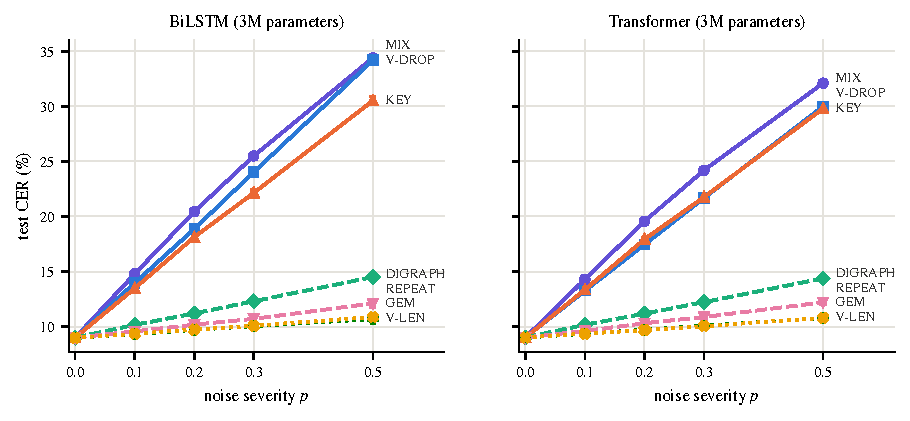
\includegraphics[width=\textwidth]{fig_noise_curves}
\caption{Test CER of the 3M models against noise severity for the seven operators. Vowel dropping, keyboard slips and mixed noise damage the models far more than vowel-length, doubled-consonant and stretching noise. Error bars: sd over five seeds.}
\label{fig:noise}
\end{figure*}

\subsection{RQ2: which training remedy helps?}
The comparison is in \Cref{tab:c2} and \Cref{fig:augmentation} (end of this section).
\textbf{Noise training buys robustness and costs clean accuracy.}
Random noise (A1) and Tamil-phonological noise (A2) lower mixed-noise CER by 2.3 and 3.0 for the BiLSTM (1.8 each for the Transformer) but add 0.8 to 0.9 clean CER, more than the 0.5 budget we set in advance.
Some of this cost may come from stopping on clean development CER, which favours the clean model.

\textbf{Tamil-aware noise helps only for what it models.}
A2 beats A1 on vowel dropping (17.7 against 21.7, BiLSTM) but loses on keyboard slips (23.4 against 18.6), which A2 does not model.
For the Transformer the two are indistinguishable on mixed noise ($-0.03$, CI $[-0.32,+0.27]$).

\textbf{Extra words, not spelling variety, explain the clean gain of back-transliteration.}
A3 improves clean CER over A0 (8.67 against 9.00, BiLSTM), but so does CTRL (8.64), and A3 and CTRL are indistinguishable on clean text ($+0.03$, CI $[-0.08,+0.13]$).
The sampled variants add a small robustness gain on mixed noise ($-0.58$ BiLSTM, $-0.81$ Transformer).
Sampled variants come from a model trained on Dakshina, so they reproduce Dakshina-style variation and not chat-style variation; a larger effect may need variants drawn from real typing.

\textbf{The combination is best.}
A4 has the lowest mixed-noise CER for both architectures (21.8) and removes most of A2's clean cost (+0.35 BiLSTM, $-0.03$ Transformer).
Our design has no ``A2 plus control'' condition, so we cannot say how much of A4's noise gain is due to varied romanizations and how much to extra words.

\textbf{Independent sets.}
On AK-all, A1 and A2 are worse than A0 (13.7 and 12.7 against 11.7, BiLSTM), while A3, CTRL and A4 are better or equal (10.8, 10.7 and 11.3).
The A3 and CTRL words come from the same kind of list as Aksharantar, so part of that gain may be vocabulary overlap rather than robustness.
Kruskal--Wallis tests over the six conditions are significant on clean and mixed noise for both architectures ($\eta^2=0.88$ to $0.93$); Dunn's test with Holm correction separates the noise-only conditions (A1, A2) from the data-rich ones (A3, CTRL) on clean text, and A4 from A0 and CTRL on mixed noise.
Neighbouring conditions, such as A1 and A2 for the Transformer, are not separated with five seeds.

\subsection{Does robustness transfer to unseen noise?}
Leaving vowel dropping out of A2 removes almost all of its benefit: BiLSTM V-DROP CER is 24.97 against 17.70 for full A2, slightly worse than the clean baseline A0 (24.03); the Transformer shows the same pattern (22.35 against 17.43 and 21.65; \Cref{fig:heldout}).
Leaving out GEM costs only 0.15 to 0.23 CER on GEM, but GEM is mild to begin with.
A model trained on one error type does not become robust to another, as Belinkov and Bisk found for natural language noise~\cite{belinkov2018synthetic}.
Practical systems therefore need operators that cover the phenomena users produce; the benchmark is a way to check that coverage, not a substitute for real data.

\begin{figure}[t]
\centering
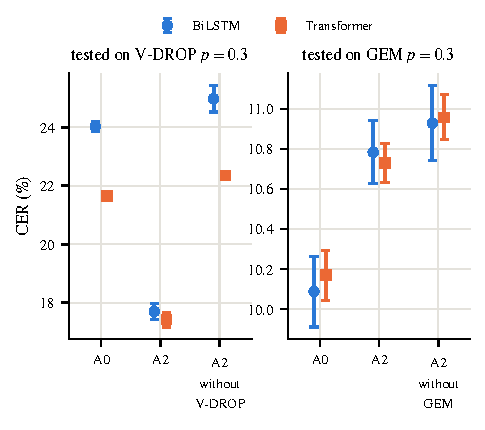
\includegraphics[width=0.8\columnwidth]{fig_heldout}
\caption{Held-out operators. Removing V-DROP from A2's training removes its benefit on V-DROP; removing GEM changes little.}
\label{fig:heldout}
\end{figure}

\subsection{RQ3: which architecture degrades less?}
Under mixed noise at $p{=}0.3$ the Transformer is better at every size (BiLSTM minus Transformer CER: $+0.42$ at 1M, $+1.30$ at 3M, $+0.28$ at 8M; \Cref{tab:stats}) and also degrades less in relative terms (+168\% against +183\% at 3M).
On clean text the BiLSTM is equal or better.
The gaps are 0.3 to 1.3 CER, the same order as the effects of tuning and seed, so we do not claim that the Transformer is generally more robust; we claim that with 20 tuned trials per cell and five seeds the architectures tie at 3M on clean text, which is consistent with the conflicting earlier rankings being a matter of tuning and seeds~\cite{wu2021applying,moran2020effective}.
Transformers were also more sensitive to hyperparameters in our tuning.

\subsection{Deployment model and a preliminary real-chat check}
\Cref{tab:v2} compares the fine-tuned model (v2) with the A4 model it started from (v1).
Clean accuracy is unchanged within noise (test CER 8.93 against 9.02; top-1 +1.4 points; top-5 $-0.2$), the independent Aksharantar sets improve slightly (AK-all 10.76 against 10.95), and robustness improves strongly: mixed-noise CER at $p{=}0.3$ falls from 21.80 to 17.77 and keyboard-slip CER from 23.04 to 15.40.
These noise gains are \emph{not} held-out evidence: the fine-tuning mixture contains all six operators, including KEY and REPEAT that A2 lacked, so the gain shows what the model learned to ignore, not generalisation.
The 2.1M mined pairs give a much smaller clean gain than extra words did in the controlled experiments, which suggests that mined romanizations resemble the existing formal data; this is an inference.

We also scored both models on 370 words from the first author's private chat exports, labelled with Tamil spellings by a language model.
\emph{These labels are not verified by a person}, so the result is indicative only.
CER is 25.4 for v1 and 24.9 for v2 (top-1 40.5\% and 39.7\%; top-5 68.6\% and 71.1\%): indistinguishable, and close to our heavy synthetic noise ($p{=}0.3$ mixed: 18--24) rather than the clean 9.
Colloquial spellings such as \emph{poren} (\tamil{போறேன்}) are the typical failures, because mined and Wikipedia-style training text uses literary forms.
Whether synthetic noise predicts real typing remains open.

\subsection{Threats to validity}
(i)~All controlled noise is synthetic and applied to formal romanizations, and operator rates come from the literature and a heuristic count on public comments, so we speak of informal \emph{romanized} Tamil and make no claim about chat text.
(ii)~Hyperparameters were tuned once per architecture and size on clean development CER with one seed, and noise-trained conditions reuse them, which disadvantages them.
(iii)~Five seeds give low power for small differences, and parameter counts match only approximately.
(iv)~Back-transliterated pairs are machine-made.
(v)~A supervisor bug started duplicate workers, so 33 of the first 72 augmentation runs shared a checkpoint folder with a duplicate process; re-scoring all 110 stored checkpoints found one that did not reproduce its logged result (8.43 against 8.49), which we retrained, and the other 109 matched to within 0.05 CER.
(vi)~Models are word-level with no sentence context, and Dakshina's Tamil lexicon contains about 0.35\% bad pairs.
(vii)~The chat words come from private conversations; only distinct lowercase words with counts were extracted, the list stays on the author's machine, and only aggregate scores are reported.

\subsection{Summary comparison}
\Cref{tab:c3,tab:c2,tab:stats,tab:v2} and \Cref{fig:augmentation} collect the comparisons discussed above.

\begin{table}[t]
\caption{Clean results (mean $\pm$ sd over five seeds). Dev and test CER in \%, beam 10; top-1 and top-5 are test accuracies. Bold: lowest test CER.}
\label{tab:c3}
\centering\scriptsize
\setlength{\tabcolsep}{3pt}
\resizebox{\columnwidth}{!}{\begin{tabular}{llrcccc}
\toprule
Model & Size & Params & Dev CER & Test CER & Top-1 (\%) & Top-5 (\%) \\
\midrule
BiLSTM & 1M & 0.98M & 8.39\,{\scriptsize$\pm$0.11} & 8.90\,{\scriptsize$\pm$0.24} & 63.6\,{\scriptsize$\pm$0.5} & 82.5\,{\scriptsize$\pm$0.4} \\
BiLSTM & 3M & 2.99M & 8.41\,{\scriptsize$\pm$0.12} & 9.00\,{\scriptsize$\pm$0.20} & 63.3\,{\scriptsize$\pm$0.2} & 82.3\,{\scriptsize$\pm$0.4} \\
BiLSTM & 8M & 8.04M & 8.43\,{\scriptsize$\pm$0.06} & \textbf{8.77\,{\scriptsize$\pm$0.07}} & 63.4\,{\scriptsize$\pm$0.2} & 83.0\,{\scriptsize$\pm$0.4} \\
\midrule
Transformer & 1M & 0.80M & 9.06\,{\scriptsize$\pm$0.13} & 9.71\,{\scriptsize$\pm$0.12} & 60.2\,{\scriptsize$\pm$0.9} & 82.8\,{\scriptsize$\pm$0.2} \\
Transformer & 3M & 3.15M & 8.49\,{\scriptsize$\pm$0.03} & 9.01\,{\scriptsize$\pm$0.17} & 63.1\,{\scriptsize$\pm$0.7} & 83.4\,{\scriptsize$\pm$0.4} \\
Transformer & 8M & 8.70M & 8.76\,{\scriptsize$\pm$0.32} & 9.40\,{\scriptsize$\pm$0.40} & 61.4\,{\scriptsize$\pm$2.0} & 83.3\,{\scriptsize$\pm$0.4} \\
\bottomrule
\end{tabular}}
\end{table}

\begin{table}[t]
\caption{Paired bootstrap over 6{,}833 test items (10{,}000 resamples). $\Delta$CER = CER($a$) $-$ CER($b$); negative favours $a$. Intervals that exclude zero are real for this test set, not necessarily for the population of trained models.}
\label{tab:stats}
\centering\scriptsize
\resizebox{\columnwidth}{!}{\begin{tabular}{llcc}
\toprule
System $a$ vs.\ $b$ & Suite & $\Delta$CER ($a-b$) & 95\% CI \\
\midrule
BiLSTM 3M vs.\ Trans. 3M & clean & -0.01 & [-0.15, +0.12] \\
BiLSTM 3M vs.\ Trans. 3M & MIX $p{=}0.3$ & +1.30 & [+1.08, +1.53] \\
BiLSTM 8M vs.\ Trans. 8M & MIX $p{=}0.3$ & +0.28 & [+0.08, +0.48] \\
BiLSTM A2 vs.\ BiLSTM A1 & MIX $p{=}0.3$ & -0.70 & [-1.00, -0.41] \\
Trans. A2 vs.\ Trans. A1 & MIX $p{=}0.3$ & -0.03 & [-0.32, +0.27] \\
BiLSTM A3 vs.\ BiLSTM CTRL & clean & +0.03 & [-0.08, +0.13] \\
BiLSTM A3 vs.\ BiLSTM CTRL & MIX $p{=}0.3$ & -0.58 & [-0.75, -0.42] \\
Trans. A3 vs.\ Trans. CTRL & MIX $p{=}0.3$ & -0.81 & [-0.95, -0.66] \\
BiLSTM A4 vs.\ BiLSTM A2 & clean & -0.48 & [-0.62, -0.35] \\
Trans. A4 vs.\ Trans. A2 & clean & -0.83 & [-0.98, -0.68] \\
\bottomrule
\end{tabular}}
\end{table}

\begin{table*}[t]
\caption{Training conditions at 3M parameters: test CER (\%) on clean text, mixed noise ($p{=}0.3$), vowel dropping ($p{=}0.3$), keyboard slips ($p{=}0.3$) and the independent AK-all set (mean over five seeds; sd at most 0.48; bold: lowest per column and architecture).}
\label{tab:c2}
\centering\footnotesize
\begin{tabular}{lcccccccccc}
\toprule
& \multicolumn{5}{c}{BiLSTM 3M} & \multicolumn{5}{c}{Transformer 3M} \\
\cmidrule(lr){2-6}\cmidrule(lr){7-11}
Condition & clean & MIX & V-DR. & KEY & AK & clean & MIX & V-DR. & KEY & AK \\
\midrule
A0 & 9.00 & 25.49 & 24.03 & 22.14 & 11.67 & 9.16 & 24.27 & 21.65 & 21.91 & 11.91 \\
A1 & 9.90 & 23.17 & 21.69 & \textbf{18.58} & 13.73 & 9.94 & 22.49 & 20.45 & \textbf{18.23} & 13.53 \\
A2 & 9.83 & 22.47 & 17.70 & 23.43 & 12.74 & 9.96 & 22.46 & 17.43 & 23.73 & 12.95 \\
A3 & 8.67 & 25.10 & 22.91 & 21.83 & 10.78 & \textbf{8.65} & 23.83 & 21.11 & 21.08 & \textbf{10.38} \\
A4 & 9.35 & \textbf{21.82} & \textbf{16.65} & 22.85 & 11.32 & 9.13 & \textbf{21.79} & \textbf{16.39} & 22.69 & 11.02 \\
CTRL & \textbf{8.64} & 25.68 & 23.58 & 22.09 & \textbf{10.67} & 8.67 & 24.63 & 21.70 & 21.91 & 10.40 \\
\bottomrule
\end{tabular}
\end{table*}

\begin{table}[t]
\caption{Deployment model against the A4 Transformer it was fine-tuned from (test CER in \%, beam 10, single run each).}
\label{tab:v2}
\centering\scriptsize
\resizebox{\columnwidth}{!}{\begin{tabular}{lccc}
\toprule
Test suite & v1 (A4) & v2 (fine-tuned) & $\Delta$ \\
\midrule
Dev CER & 8.47 & 8.56 & +0.10 \\
Test CER & 9.02 & 8.93 & -0.09 \\
Test top-1 (\%) & 63.88 & 65.27 & +1.39 \\
Test top-5 (\%) & 85.03 & 84.81 & -0.22 \\
AK-all CER & 10.95 & 10.76 & -0.20 \\
MIX $p{=}0.1$ CER & 13.41 & 11.89 & -1.52 \\
MIX $p{=}0.3$ CER & 21.80 & 17.77 & -4.03 \\
MIX $p{=}0.5$ CER & 28.79 & 23.02 & -5.77 \\
V-DROP $p{=}0.3$ CER & 16.20 & 16.00 & -0.20 \\
KEY $p{=}0.3$ CER & 23.04 & 15.40 & -7.63 \\
REPEAT $p{=}0.3$ CER & 10.97 & 9.51 & -1.46 \\
\bottomrule
\end{tabular}}
\end{table}

\begin{figure*}[t]
\centering
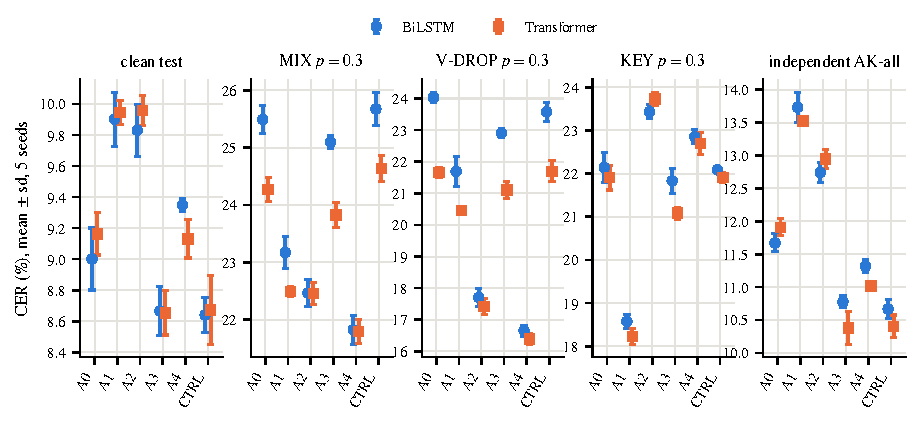
\includegraphics[width=\textwidth]{fig_augmentation}
\caption{Training conditions: test CER on clean text, three noise suites and the independent AK-all set (mean $\pm$ sd over five seeds).}
\label{fig:augmentation}
\end{figure*}

%% ------------------------------------------------------------------
\section{Conclusion}
We built a paired, seeded robustness benchmark for Latin-to-Tamil word transliteration and used 110 trained models to measure it.
Informal typing hurts mainly through dropped vowels and key slips; Tamil-aware noise training removes much of the vowel-drop damage but not damage from operators it does not model; extra romanized words matter at least as much as spelling variety, and combining Tamil-phonological noise with back-transliterated data is the best overall at no clean cost; and the BiLSTM and the Transformer are close, with the Transformer slightly better under heavy noise.
Our implementation reproduces the published Dakshina baselines.

\textbf{Future work.}
The next step is verified real typing: a hand-checked chat word set and a team-typed set, to show whether synthetic noise predicts real degradation.
Other directions are lexicon and language-model reranking on noisy input, variants sampled from real typing, byte-level pretrained models and sentence context.

\textbf{Reproducibility.}
Code, configurations, per-run logs, result summaries and the scripts that generate every table and figure are in the project repository (\texttt{github.com/lebiraja/tamil-translit-robustness}, private until release); Dakshina and Aksharantar are available from their original sources, and the noisy test sets are regenerated deterministically by the repository scripts.

\printbibliography

\end{document}
